\documentclass{article}

% IMPORT PACKAGES
\usepackage{graphicx}
\graphicspath{{images/}}
\usepackage{blindtext}
\usepackage[T1]{fontenc}
\usepackage[latin9]{inputenc}
\usepackage[a4paper]{geometry}
\geometry{verbose,tmargin=2cm,bmargin=2cm,lmargin=1cm,rmargin=1cm}
\setlength{\parskip}{\smallskipamount}
\setlength{\parindent}{0pt}
\usepackage{array}
\usepackage{mathtools}
\usepackage{dsfont}
\usepackage{amsmath}
\usepackage{amssymb}
\usepackage{lmodern}
\usepackage{eqlist}
\usepackage{babel}
\usepackage{multicol}
\usepackage{stackengine}
\usepackage{xcolor}
\usepackage{listings}
\usepackage{subcaption}
\usepackage{float}
% BLOCKS
\usepackage{beamerarticle}
\usepackage[most]{tcolorbox}
%	COMMON COLORS
\definecolor{_light_green}{rgb}{0.36, 0.84, 0.36}
\definecolor{_light_grey}{rgb}{0.90, 0.90, 0.90}
\definecolor{_white}{rgb}{1.0, 1.0, 1.0}
\definecolor{_blue}{rgb}{0.0, 0.0, 1.0}
\definecolor{_light_blue}{rgb}{0.7, 0.9, 1.0}
%	DEFINE BOXES
\newtcolorbox{_block}[1][]{
    colbacktitle=_light_grey,		% title background
    coltitle=black,					% title color
    titlerule=0pt,
    colback=white!50!_light_grey,	% body background
    boxrule=0.4pt,					% content-frame padding (or frame width)
    colframe=black!20!_light_grey,	% frame color
    left=0mm,						% content and title left padding
    arc=0.5pt,						% border-radius
    title={#1},
}
\newtcolorbox{_example}[1][]{
    colbacktitle=_light_green,
    coltitle=black,
    titlerule=0pt,
    colback=white!60!_light_green,
    boxrule=0pt,
    colframe=white,
    left=0mm,
    arc=0.5pt,
    title={#1},
}
\newtcolorbox{_note}[1][]{
    colbacktitle=_light_blue,
    coltitle=black,
    titlerule=0pt,
    colback=white!60!_light_blue,
    boxrule=0pt,
    colframe=white,
    left=0mm,
    arc=0.5pt,
    title={#1},
}
\newtcolorbox{_block_emph}[1][]{
    enhanced,
    frame hidden,
    borderline west={2.0pt}{0pt}{blue!60!white},
    opacityframe=0.0,
    colback=blue!4!white,
    left=2mm,
    arc=0.5pt,
    title={#1},
}
%   CUSTOM CODE LISTINGS
\newtcblisting{code}[2][]{
	colback=blue!5!white,
	colframe=red!75!black,
	opacityframe=0.0,
	coltitle=black,
	left=5pt,
	lefttitle=0pt,
	enhanced,
	listing only,
	title=\textbf{#2},
	arc=0.5pt,
	listing engine=minted,
	minted language={#1},
	minted style=colorful,
	minted options={
		fontfamily=\sfdefault,%\sserif
		fontsize=\scriptsize,
		breaklines,
		autogobble, %linenos, %numbersep=1mm,
		tabsize=4,
		escapeinside=||,mathescape=true,
	},
	overlay={
		\begin{tcbclipinterior}
			\fill[black!30!white] (frame.south west) 
			rectangle ([xshift=1mm]frame.north west);
		\end{tcbclipinterior}
	},
}

% below command to set inline code style doesn't work    :(
\lstset{language=C,keywordstyle={\bfseries \color{blue}}}

% \usepackage{subfiles}
% \subfile{}

% DOCUMENT

\begin{document}

% short title:
%   \part*{}
%   \part[]{}

\title{CS3237 Introduction to Internet of Things \\ Group 4 Report}
\author{Lai Yu Heem, Pinkl Constantin Maxime, Teo Chuan Kai, Wong Chee Hong, Thomm Leon Felix}
\maketitle

% changing sections enumeration style
% styles: \arabic{} \alph{} \Alph{} \roman{} \Roman{}
\renewcommand\thesection{\arabic{section}}
\renewcommand\thesubsection{\thesection.\alph{subsection}}

\newcommand\ISquaredC{$\text{I}^2\text{C}$}

\section{Abstract}

In this reoprt we describe the construction and implementation of an IoT device that forecasts under water weather conditions. The device and all its components are put into a water-proof, floating box i.e. a buoy. A WeMOS micro-controller is the heart of the device which collects wave movement data through an accelerometer and gyroscope. Additionally, other relevant data such temperature and turbidity data is also gathered to make good predictions. A phone with our own app serves as the gateway to a cloud back-end infrastructure. In the cloud, we store previous recorded data for visualisation and training purposes of the ML Model which is able to provide a score that represents diving suitability.

\section{Introduction}
\begin{multicols}{2}
Weather forecasts are part of our everyday life, however most of them are only made for above weather conditions. This is understandable since most people are only concerned with how weather will be above sea level. Additionally, under-sea weather may be very localized to a certain, specific body of water. Nevertheless, there still exists many cases where it is crucial to know the conditions under water in the near future.

For some busy locations (e.g. Singapore) there might be systems implemented that predict future water conditions, however, these forecasts are also needed in less developed countries and less busy sites. Therefore, we found the need for a low cost, easy-to-deploy system that can provide an accurate short-term forecast about future under-sea conditions after a sufficient training on localised conditions.

In this project, we focused specifically on providing a diving score which provides an indication of the underwater conditions relevant for scuba diving, allowing divers to better plan based on the conditions forecast. Here, it is important to mention that such a score does not exist yet, especially specifically for scuba diving. Therefore, we provide a score relative to a baseline which we define as good diving conditions.

\end{multicols}

\section{Solution Approach}

\begin{multicols}{2}
    To provide a picture of the diving conditions in a localised area, we devised a buoy housing multiple sensors to capture relevant maritime data. A buoy can provide accurate information about its immediate vicinity. A fleet of buoys scattered across a large area can provide a bigger picture of ocean conditions in the area of interest. With the large volume of data from the buoys, we can provide diving score for a given area in the ocean.
    \begin{center}
        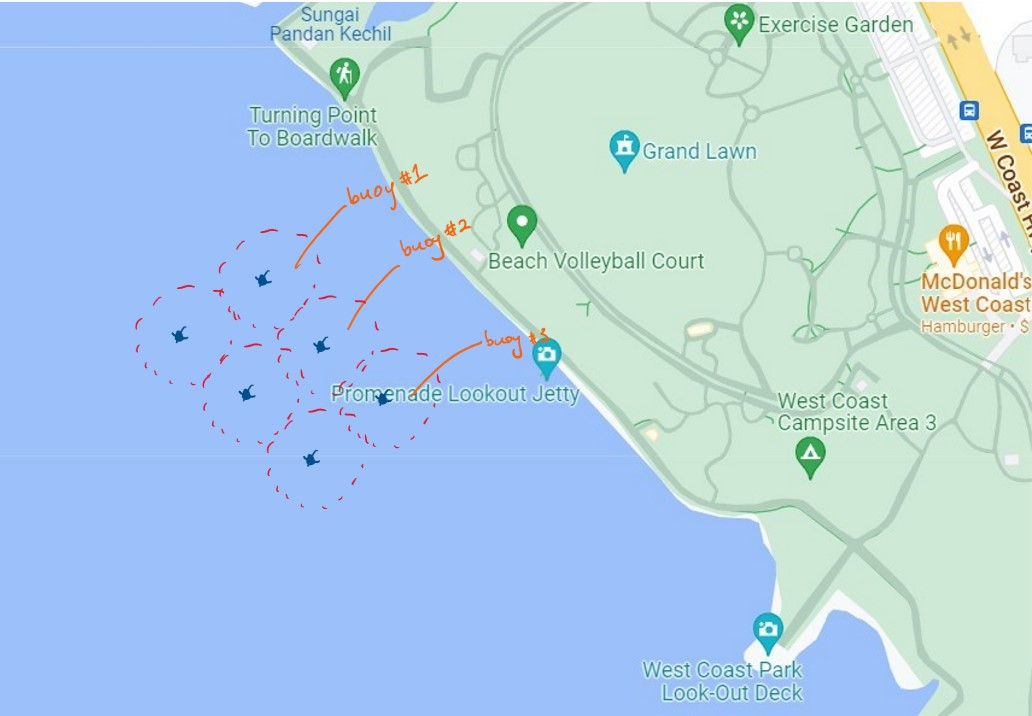
\includegraphics[width=\columnwidth]{report/images/buoy-fleet.jpg}
        \textsc{Buoy Fleet}
    \end{center}
\end{multicols}

\newpage
\subsection{Architecture overview}

\begin{multicols}{2}

Physically, the system consists of two components: the \textit{cloud} and the \textit{buoy(s)}, whereas a buoy can be further divided into \textit{WeMOS} and \textit{phone}. 

The WeMOS collects most of the data of interest (temperature, wave movement, water turbidity) through sensors. It then sends collected records to the phone via WiFi, which extends it and timestamps the data collected. The phone also serves as a gateway and forwards the records to the server running in the cloud. These functions within the phone are powered by a custom application, which buffers information from the WeMOS, before sending them in batches to the server for processing.

The cloud aspect of the architecture serves two key function within our solution. First, it acts as a central repository of data collected from sensors within our buoy. This data is then used to train our machine learning (ML) model, and for calculating the short-term forecast of the underwater conditions. Second, the cloud also hosts a front-end for our target audience such as scuba divers to access information and forecasts derived from our buoys through our pre trained ML models.

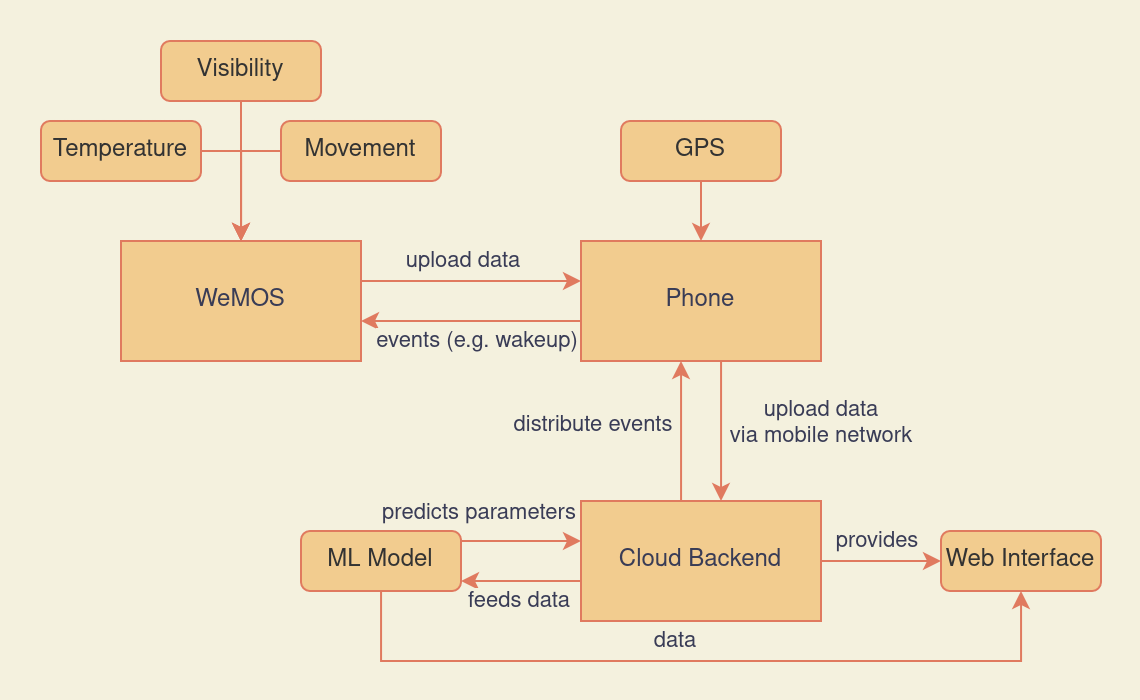
\includegraphics[width=\columnwidth]{report/resources/architecture.png}

\end{multicols}

\subsection{Buoy Hardware}

\begin{multicols}{2}

The WeMOS collects most of the data. In particular, we collected

\begin{itemize}
    \item water temperature
    \item wave movement (accelerometer, gyroscope)
    \item water turbidity
\end{itemize}

For temperature, we used the temperature  module from the set, sticking out of the buoy into the water. The water turbidity was implemented using an LED shining light through a section of water, and a photoresistor on the other side.

Temperature sensor and photo-resistor were connected to the ADC, and accelerometer data was supplied from the MPU. Both ADC and MPU communicate with the WeMOS over \ISquaredC.

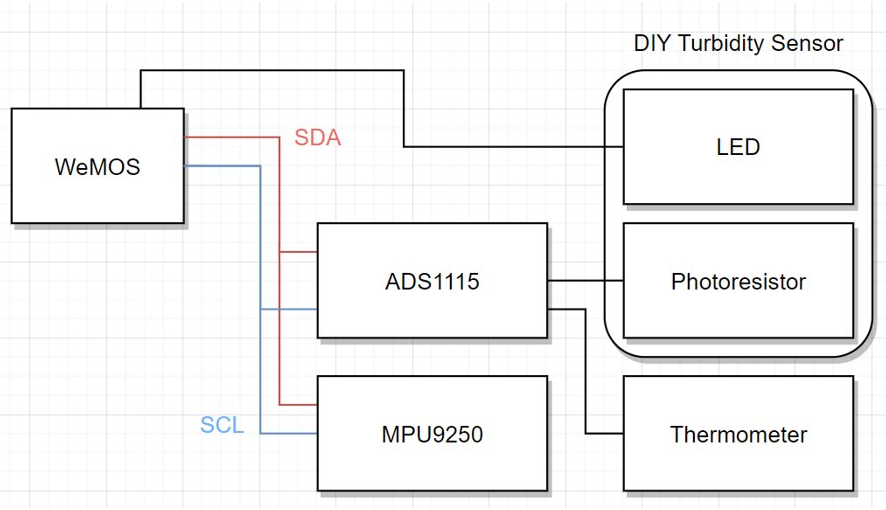
\includegraphics[width=\columnwidth]{report/images/wiring.png}

\end{multicols}

\subsection{Phone applications}

\subsubsection{General Concept}
\begin{multicols}{2}
The phone acts as a middle man between the cloud and the WeMOS and is placed within the buoy itself. During testing and debugging, the phone provided us with a clean user interface to inspect the data coming the WeMOS itself. Given that we plan to scale the system into a fleet of buoys, GPS data is necessary to pinpoint the exact location of each buoy. As such, the phone provides GPS data for each buoy as well. Data measurements from the WeMOS and the sensors are sent to the phone through a socket connection and the phone then appends a timestamp and GPS to each data received. To preserve battery on the phone, we buffer a certain number of measurements before sending them in a single batch to the cloud. Phone-Cloud communication is done via MQTT.
\begin{figure}[H]
    \centering
    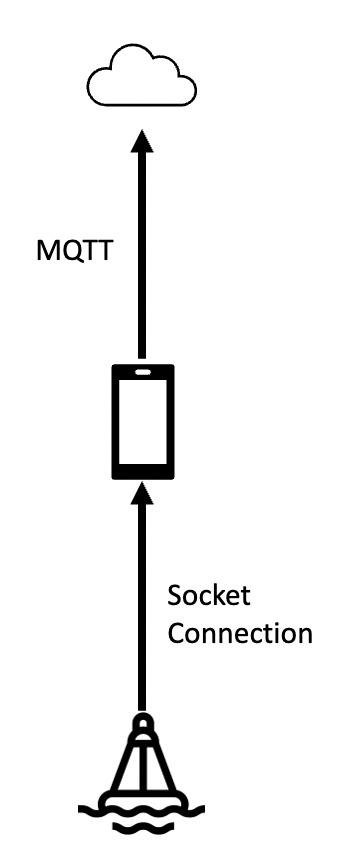
\includegraphics[height=8cm]{report/images/phone_app_concept.png}
    
    \label{fig:my_label}
\end{figure}
% \begin{center}
%     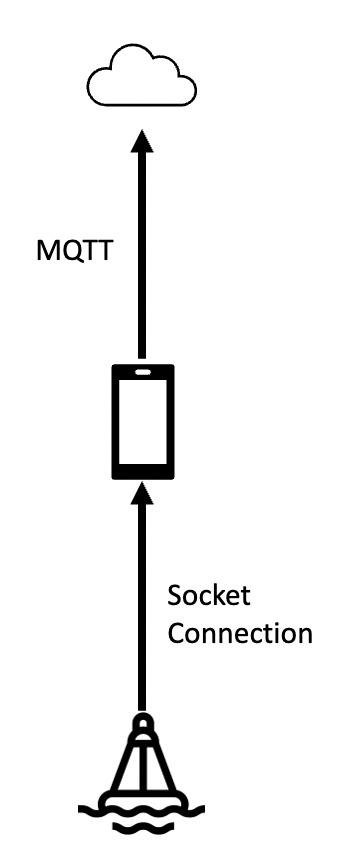
\includegraphics[height=8cm]{report/images/phone_app_concept.png}
% \end{center}
\end{multicols}


\subsubsection{Phone App Framework}
\begin{multicols}{2}
 The phone app is written in Dart using the Flutter framework by Google. Flutter allowed us to develop on both Android and IOS devices using the same source code, reducing code duplication. Furthermore, the rich libraries available in Flutter allowed us to implement socket communication with the WeMos and MQTT communications with the cloud server with ease. Exact implementation details will be discussed below.
\columnbreak


\begin{center}
    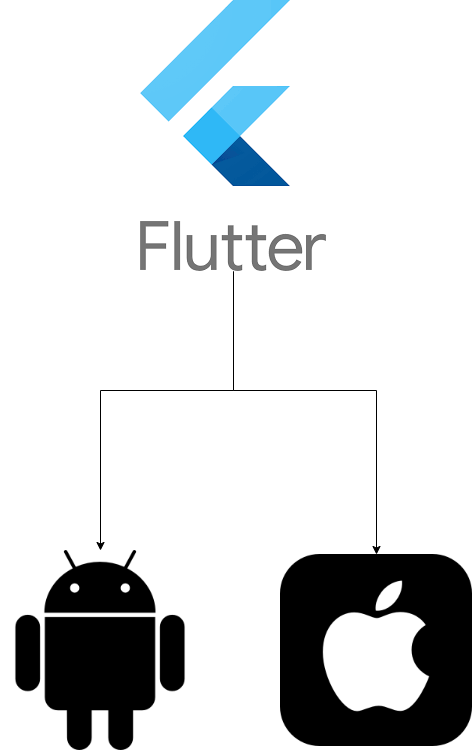
\includegraphics[height=5cm]{report/images/dart-a-ios.drawio.png}\\
    \textsc{Build Pipeline of Flutter\\Icon Source: Flaticon.com}
\end{center}
%<a href="https://www.flaticon.com/free-icons/logo" title="logo icons">Logo icons created by Pixel perfect - Flaticon</a>
% <a href="https://www.flaticon.com/free-icons/android" title="android icons">Android icons created by Freepik - Flaticon</a>


\end{multicols}
\textbf{Socket Connection}
\begin{multicols}{2}
\begin{code}[dart]{Setup Socket}
final server = await ServerSocket.bind("192.168.43.1", 4567); 
server.listen((client) {
   handleConnection(client);
});
\end{code}
\columnbreak

\begin{code}[d]{Phone Dart Code}
void handleConnection(Socket client) {
    client.listen(
    	(Uint8List data) async {
     	 final message = String.fromCharCodes(data);
    	},
   	onError: (error) {
    	  client.close();
   	 },
   	 onDone: () {
     	 client.close();
    	},
  );
}  
\end{code}
\end{multicols}
\begin{multicols}{2}
We can use these two snippets to setup our connection with our phone. As soon as the WeMOS establishes internet connection with the phone's hotspot connection, it will attempt to establish socket communication with the phone before collecting data. Upon establishing the socket server, the WeMOS performs a time-sync with the phone application. We are required to do that since the WeMOS itself does not have a real-time clock. Thereafter, every data measurement collected by the WeMOS is appended with the offset since the time-sync, before being sent to the phone. This gives us an accurate timestamp for each measurement. 

As mentioned before, we always buffer a certain amount of measurements before sending it to the cloud using the MQTT protocol.
\end{multicols}

\subsubsection{MQTT Connection}
\begin{multicols}{2}

\begin{code}{Setup Client}
void setup(){
    MqttServerClient mqttclient = MqttServerClient.withPort(address, 'iot_device', 1883);
    final connMessage = MqttConnectMessage()
          .authenticateAs('username', 'password')
          .withWillTopic('willtopic')
          .withWillMessage('Will message')
          .startClean()
          .withWillQos(MqttQos.atLeastOnce);
    mqttClient.connect();
}
\end{code}

\begin{code}{Publish to Topic}
void publish(String data2SendStr) {
    const pubTopic = 'topic/test';
    final builder = MqttClientPayloadBuilder();
    builder.addString(data2SendStr);
    mqttclient.publishMessage(pubTopic, MqttQos.atLeastOnce, builder.payload!);
}
\end{code}

This setup of the MQTT client only provides a one way communication from the phone to the cloud, however, this was sufficient for our project. Within the application, the "publish" method receives a string representation of the payload, and sends it to the server.
\end{multicols}

\newpage
\subsubsection{Front End}
\begin{multicols}{2}
The UI of the app is very simple. The user has two ways to interact with the application. First, a button to start the MQTT client and the socket server. Second, a button to start sending the data received. We can choose to discard the collected data before sending it if we deem the data collected to be inaccurate. Additionally to the buttons, the app displays all data packets still in the buffer. This allowed us to inspect the data before sending it to our cloud database and proved very useful for debugging.


\begin{center}
 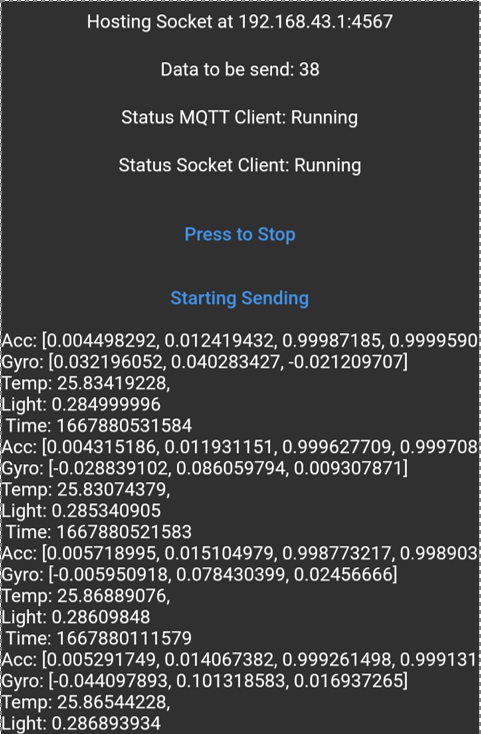
\includegraphics[height=\columnwidth]{report/images/911d517b579539015591262ca9a8d9ea.png}\\
\textsc{App sockets and MQTT running but not sending data}
\end{center}



\end{multicols}

\subsection{Server-side}

\begin{multicols}{2}

The server aspect of our implementation is powered by a DigitalOcean Droplet hosted within the cloud, accessible through the domain \texttt{iot.ckteo.com}. It serves two key functions within our proposed approach. Firstly, it acts as a central repository for data collected from the sensors within our buoys and secondly, it serves as a portal for our target users to access information and forecasts related to the specific area that the buoys are deployed in. The server consists of four key components: 
\begin{itemize}
    \item a MQTT broker - facilitating foundations for data transfer through MQTT
    \item a listener based on Python - to detect when data is published to MQTT channels and/or topics
    \item a \texttt{mongodb} nosql database - a database to store all recorded sensor data
    \item a web app based on Flask - to display information related to forecasts
\end{itemize}

Each of the components within the server is implemented as Docker containers, assisted by the \texttt{docker-compose} tool, allowing simple management of different environments, dependencies and easy migration of data. The following sub-sections will elaborate on each component hosted within the server.

\end{multicols}

\subsubsection{MQTT Broker}

\begin{multicols}{2}

An MQTT broker is set up, listening on TCP port 1883 and is exposed to the public internet. The purpose of the MQTT broker is to facilitate the infrastructure for MQTT communication between the phone within the buoy acting as the gateway, and the server within the cloud. The MQTT broker is secured with basic authentication so as to prevent malicious users from feeding erroneous data to the server.

\end{multicols}

\subsubsection{Python Listener}

\begin{multicols}{2}

Considering the design of the gateway mobile application, data collected from sensors will be published to a particular channel and topic through the MQTT broker within the cloud. The python listener program is designed to subscribe to the related MQTT channel and topics, runs a loop that listens for any incoming data published to the channel and topic, formats the data, and adds it into the MongoDB database. The design motivation behind the listener is with the goal of offloading any processing responsibility away from the gateway (mobile phone within the buoy), and towards the server. This is with the intention of minimising power consumption of the components within the buoy itself, and to minimise the impact of network latency (such as connecting and interfacing directly with the MongoDB server)

\end{multicols}

\subsubsection{MongoDB Server}

\begin{multicols}{2}

An instance of MongoDB is present within the server, acting as a central repository for historical data previously reported from the individual buoys. The MongoDB instance is not exposed to the public internet in adherence to security best practices, and is only interacted with by applications and programs residing within the server. We opted for a NoSQL, document-oriented database program as it allowed us to modify the data structures of records stored within the database, extremely beneficial as we were still undergoing phases of prototyping.

\end{multicols}

\subsubsection{Flask Web App}

\begin{multicols}{2}

A web application written in Flask is set up within the server, listening on TCP port 80, accessible through the URL \texttt{http://iot.ckteo.com}. This web application acts as an interface for users to interact with the data fed in from the buoys. It references data stored within the MongoDB instance to fulfill this feature.

\end{multicols}

\subsection{ML model and application}

\begin{multicols}{2}
Since our team wanted to make forecasts that uses historical and current data of various underwater features to predict future values, we looked at various models for time series forecasting. We ended up using Long Short-Term Memory networks (LSTM) as it was suitable for our problem which involved learning patterns of data over a time period.

We created a LSTM model that used a look-back window of size 10 and forecasts 10 steps ahead into the future. The time intervals we used were 1 second which matched the the data collection intervals from our IoT buoy so no up-sampling or down-sampling of the data was done. The data was scaled using \texttt{StandardScaler} before it was used to train our model.  We faced difficulties adjusting the shape of the layers to handle multivariate forecasts so we stuck to using training three separate models for each feature we wanted to forecast. The three main features which were being predicted were the temperature, visibility and the turbulence. The turbulence data was calculated as an aggregate of the gyroscope data as well as the accelerometer data.

The final aggregate score measures how close to our baseline conditions the forecasted conditions will be from the training data collected. Since our model was trained on relatively good and calm conditions, we made the assumption that larger deviations from this baseline would produce a worse (lower) score. Large deviations from this condition would imply that the weather was not calm and possibly stormy. The deviation was calculated by weighting the prediction for each feature made by the model. The respective weights for light, turbulence and temperature were: 0.45, 0.45 and 0.1 because we felt visibility as well as the turbulence of water were more important factors in this geographical region for diving conditions. The score was then calculated as an inverse on the deviation.

\begin{code}{Building LSTM Model}
def build_model(name, trainX, trainY):
    if os.path.exists(name):
        model = load_model(name)
    else:
        model = Sequential()
        model.add(LSTM(64, input_shape=(1,10)))
        model.add(Dense(10))
        model.compile(loss='mean_squared_error', optimizer='adam')
        model.fit(trainX, trainY, epochs=20, batch_size=1, verbose=2)
        model.save(name)
    return model
\end{code}

\begin{center}
    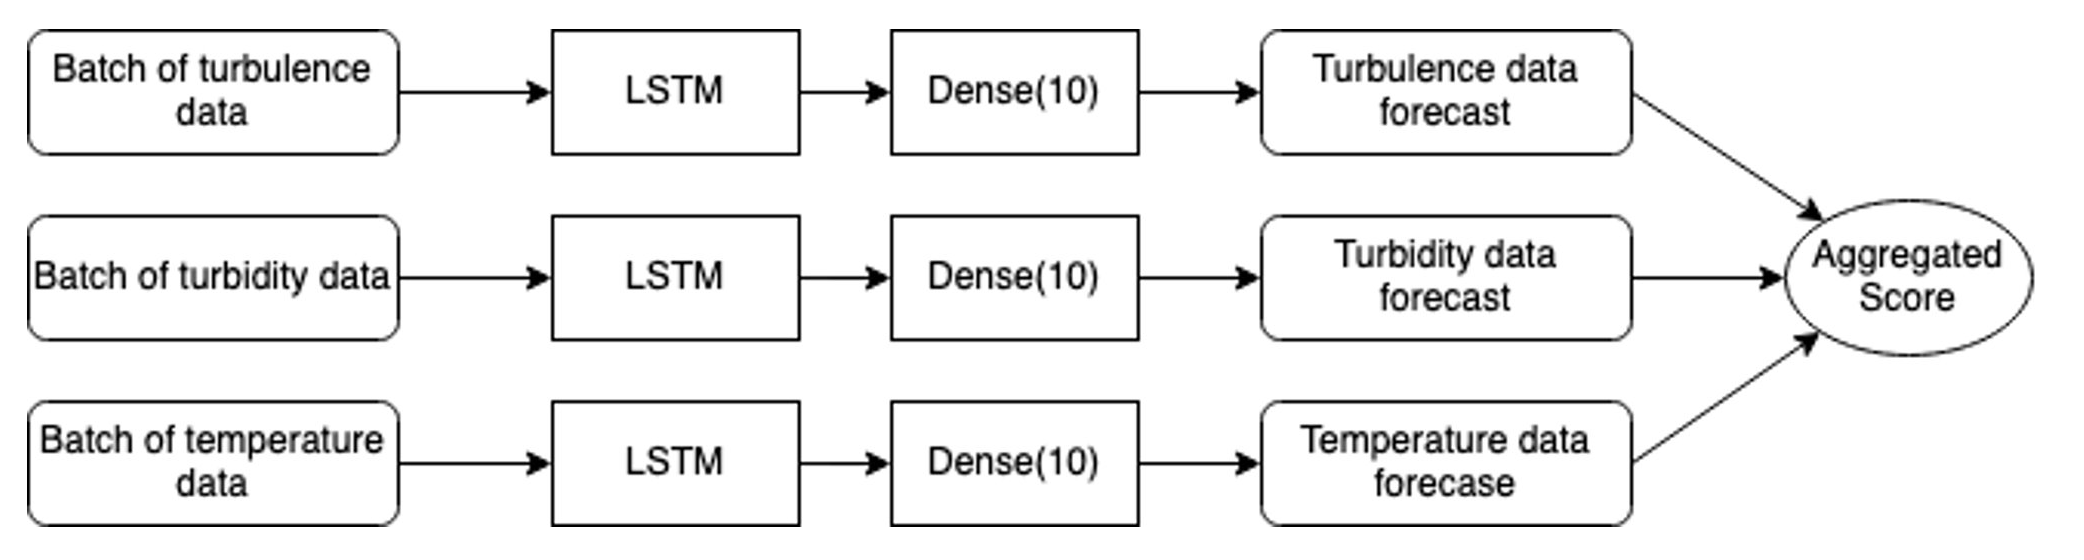
\includegraphics[width=\columnwidth]{report/images/model.png}\\
    \textsc{Model Pipeline}
\end{center}

\end{multicols}

\subsection{User interface}
\begin{multicols}{2}
    The user interface consists of two pages. First, we have a page that provides the current predicted score of how suitable the current under water weather conditions are. This score is refreshed and updated at 10 second intervals. The score shown to the user is based on the amount of deviation away from the baseline data that we have previously trained. As we were only able to collect data limited to "good" weather conditions, this score hence will reflect the amount of deviation away from the collected baseline. A lower score represents a significant deviation from the baseline "good" weather, advising divers that forecast conditions may be poor. Conversely, a higher score represents little deviation from the baseline "good" weather, advising divers that forecast under-sea conditions may be optimal for diving.

\begin{center}
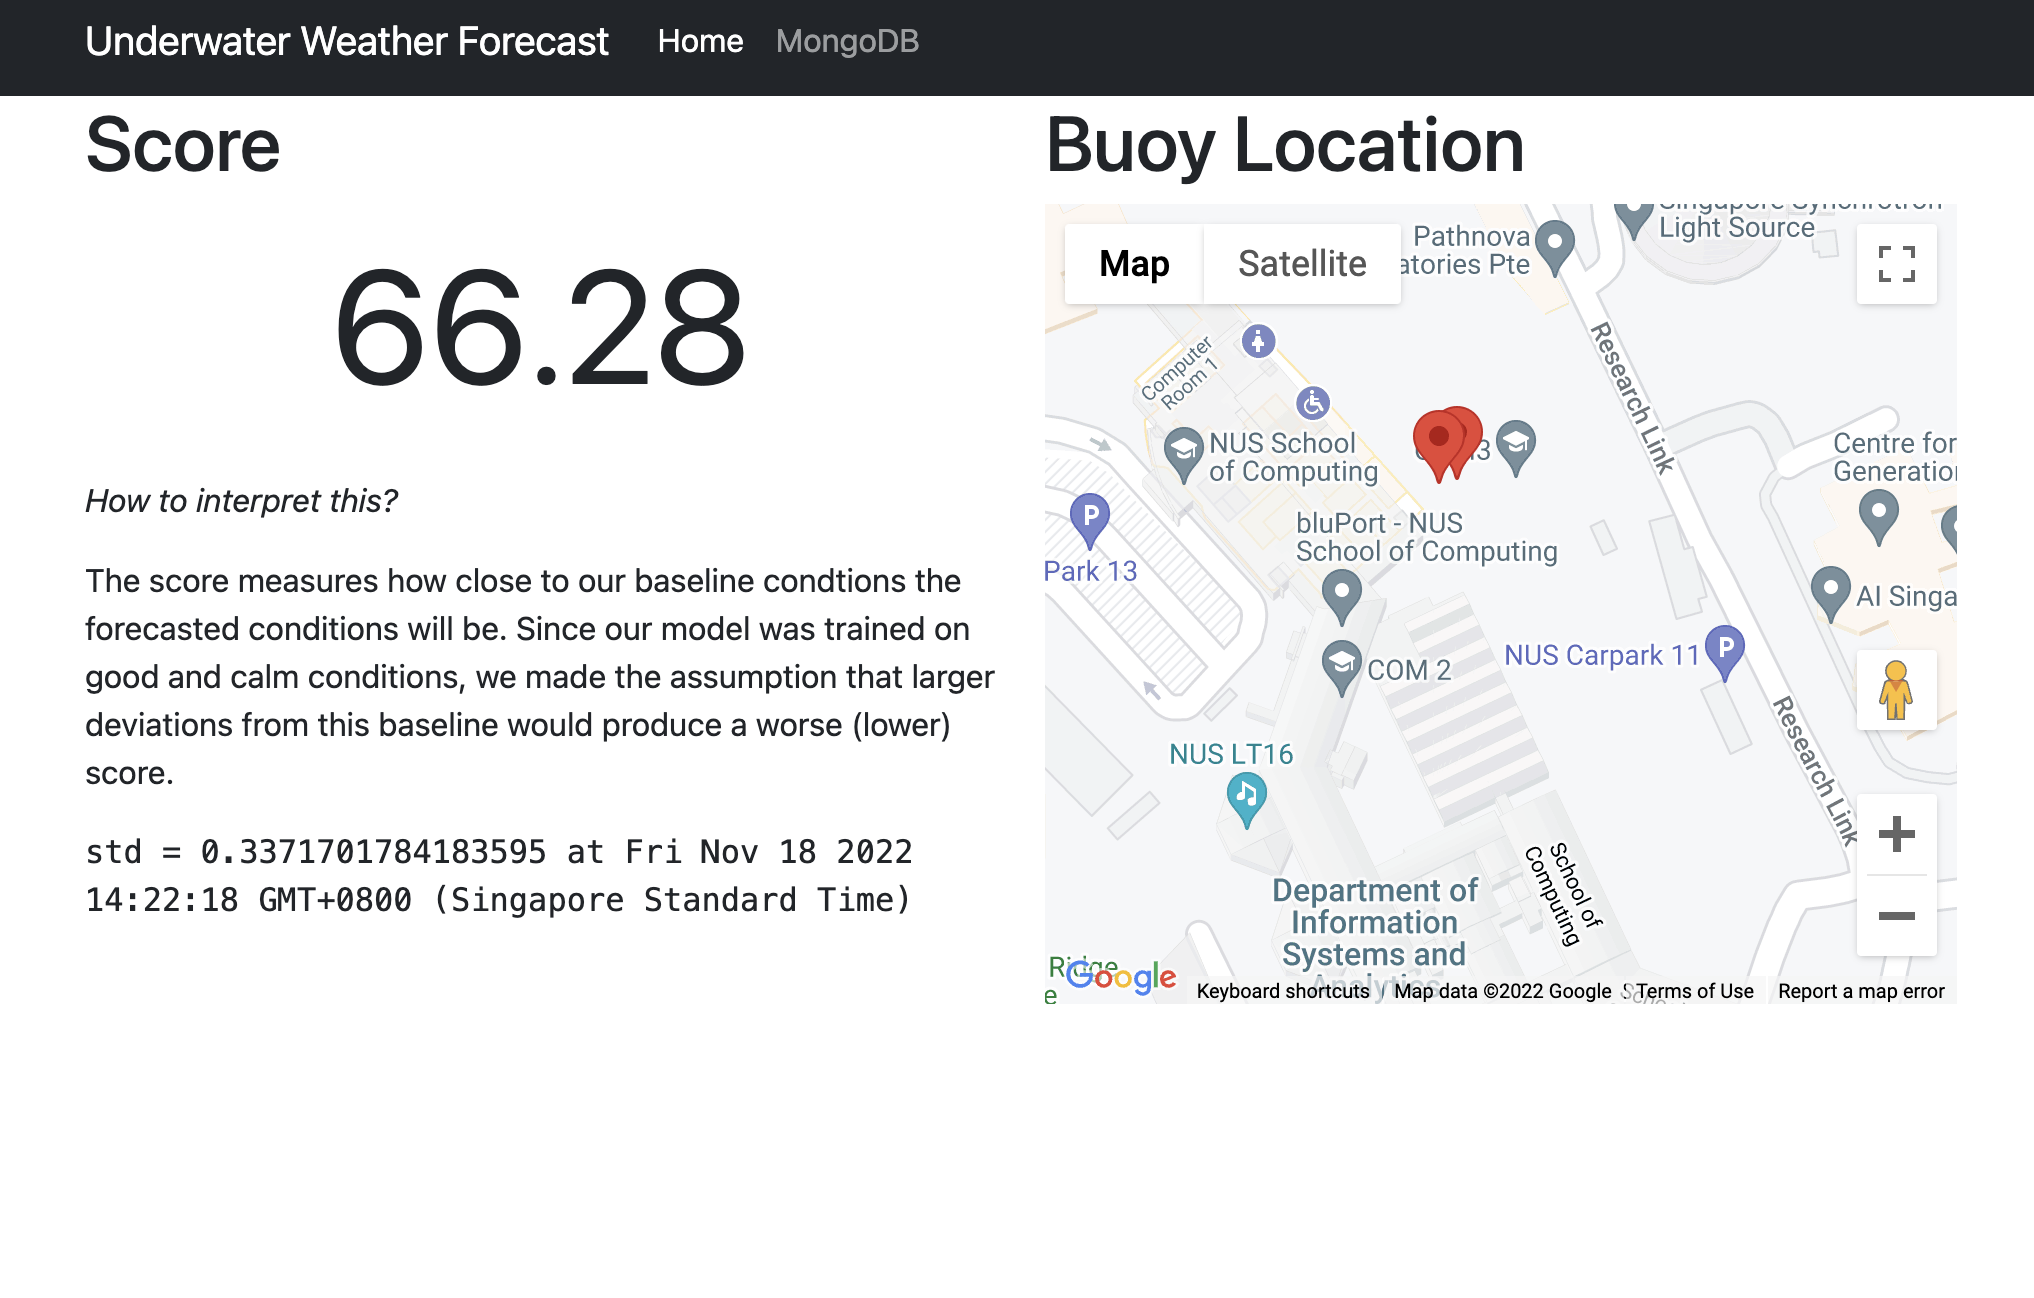
\includegraphics[width=\columnwidth,height=8cm]{report/images/score.png}
    \textsc{Current predicted score for a certain location}
\end{center}
    
\columnbreak
Second, we have a page that shows a dashboard which displays the currently collected data of all the deployed buoys for the last 15 data snapshots. The dashboard is refreshed and updated at 2 second intervals.
\begin{center}
    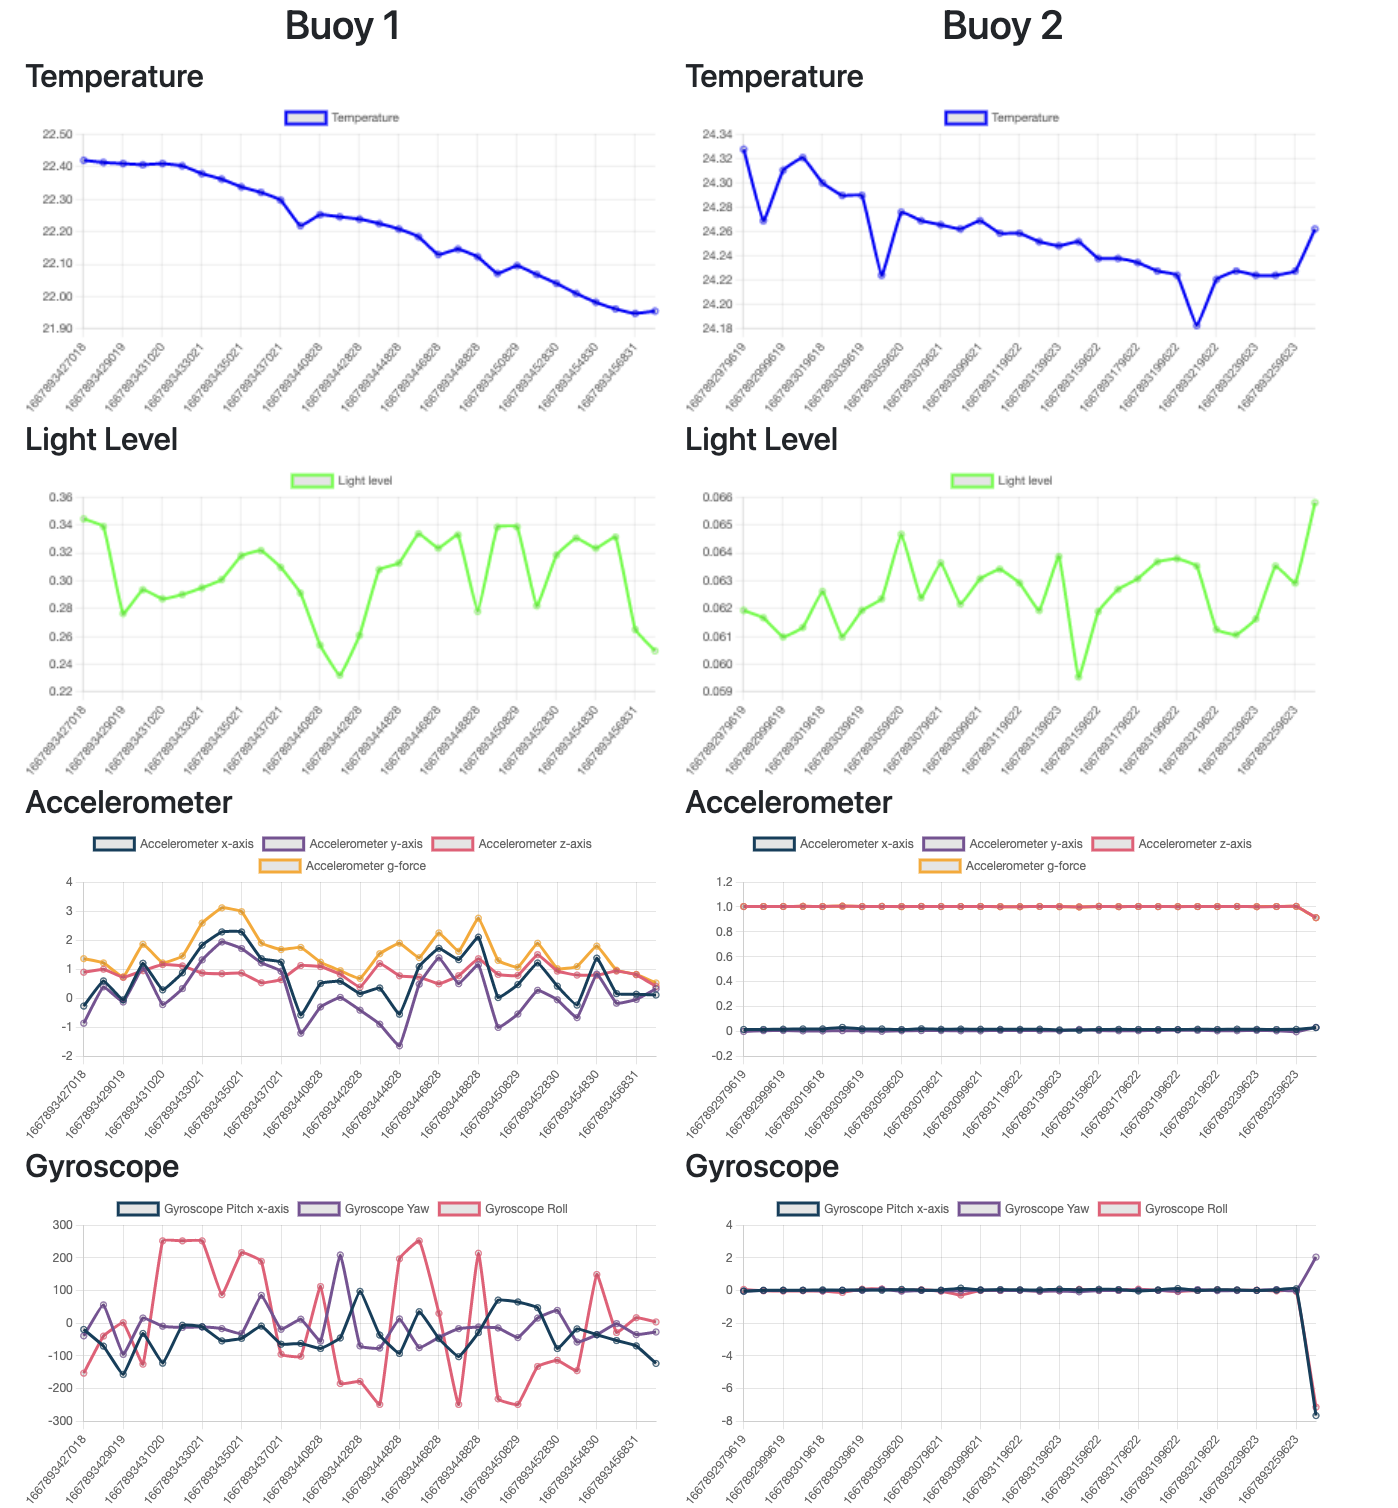
\includegraphics[width=\columnwidth]{report/images/alldata_pic.png}
    \textsc{displaying the currently measured sensor values for all Buoys}
\end{center}
   
\end{multicols}

\newpage
\section{Implementation Details}

\subsection{Buoy and Waterproofing}

\begin{multicols}{2}
A plastic lunch box with rubber seals was used to house the WeMOS, sensors and battery. Holes were drilled into the box to allow the probe of the temperature sensor to come into contact with water. A larger hole was made in the box to implement a home-made turbidity sensor. A rope was attached to the lid of the lunch box to prevent the buoy from drifting too far away when placed in the sea. All water ingress points were filled in with epoxy resin, followed by an additional layer of co-polymer sealant. 

\begin{center}
 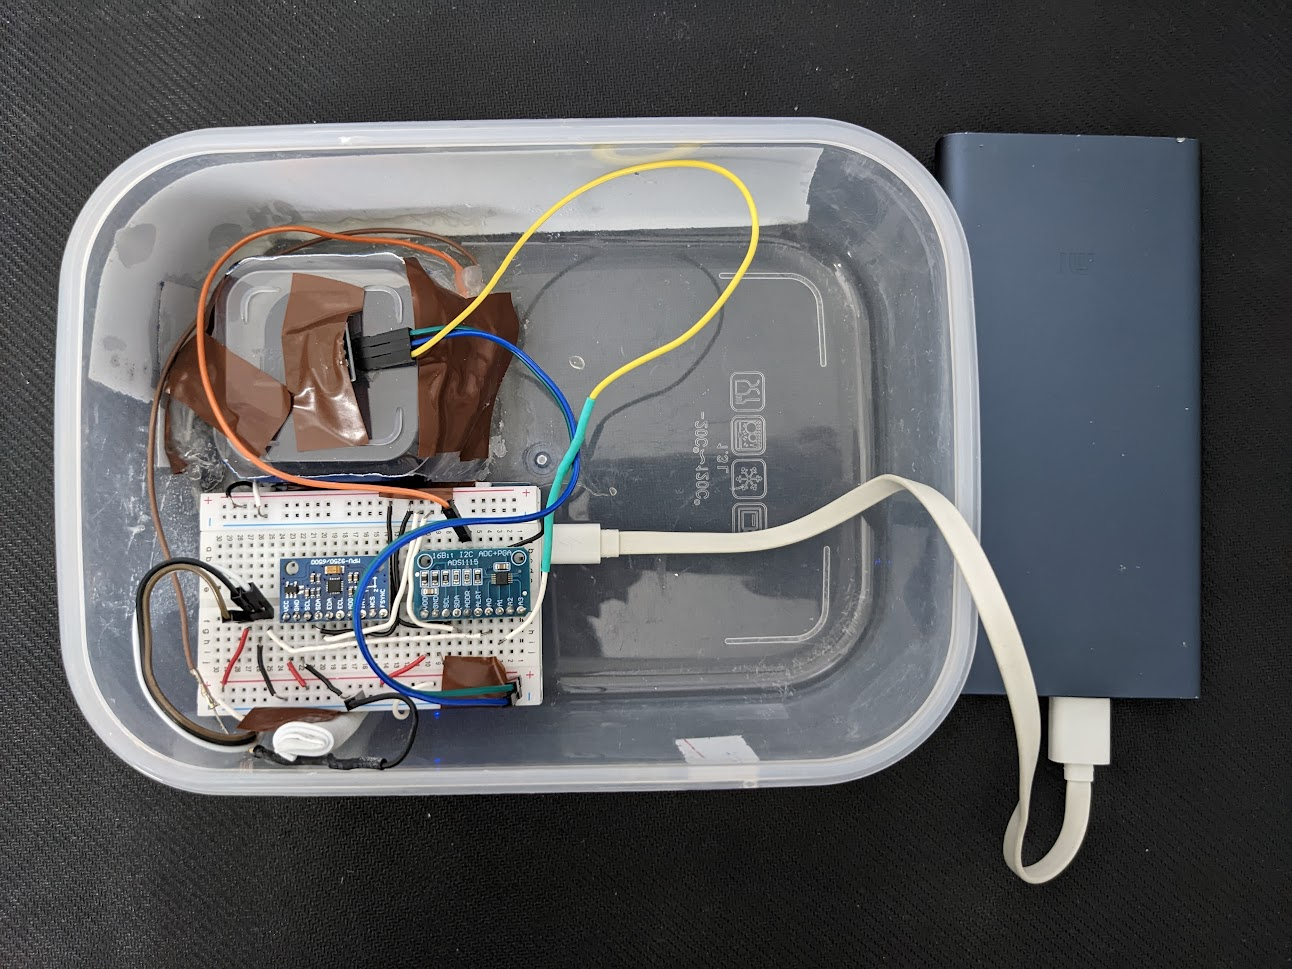
\includegraphics[width=\columnwidth]{report/images/buoy-top-view.jpg}\\
 \textsc{Top View of Buoy}
 
 \columnbreak
 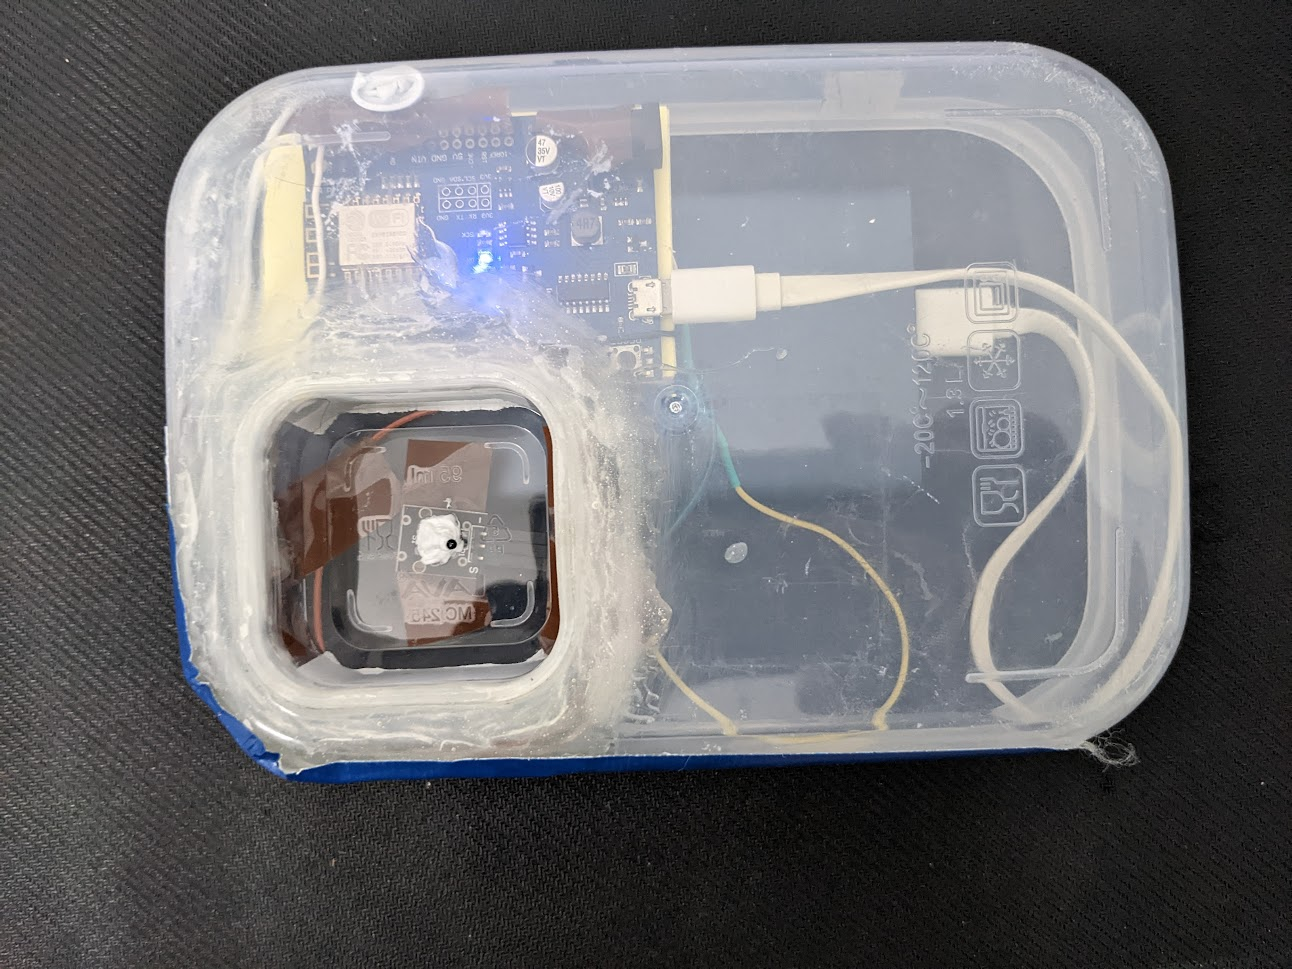
\includegraphics[width=\columnwidth]{report/images/buoy-bottom-view.jpg}\\
 \textsc{Bottom View of Buoy}
 
 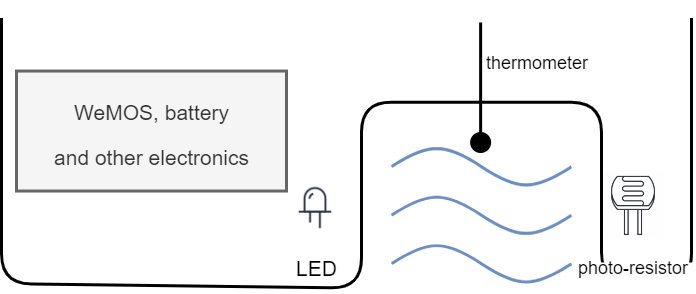
\includegraphics[width=\columnwidth]{report/images/buoy-cross-section.png}\\
 \textsc{Cross-sectional diagram of Buoy}

\end{center}


\end{multicols}

\newpage
\subsection{Turbidity sensor}

\begin{multicols}{2}
Visibility of the water is an important factor when determining diving safety. As such, a turbidity sensor is a essential element of our buoy. To measure water visibility using the box of sensors available to us, we referenced a commercially-available turbidity sensor and replicated the key principles involved in determining water visibility. Intuitively, murky water scatters and blocks light. The murkier the water, the more light it will block. By placing water in-between a light-source (such as an LED) and photo-resistor, we can measure changes in light level due to the murkiness of the water.

Our solution involved placing a square cavity into the buoy, where water can flow into. A LED and photo-resistor was then fixed on opposing ends of the cavity, as illustrated in the cross-sectional diagram in the section above.

A proof-of-concept experiment was conducted to show that our home-made turbidity sensor works. In a dark room, various concentrations of water and milk coffee were placed between the LED and photo-resistor. We were able to observe a negative correlation between the light level detected by the photo-resistor and the murkiness of the water.

\end{multicols}
\begin{figure}[H]
    \begin{subfigure}{.33\textwidth}
        \centering
        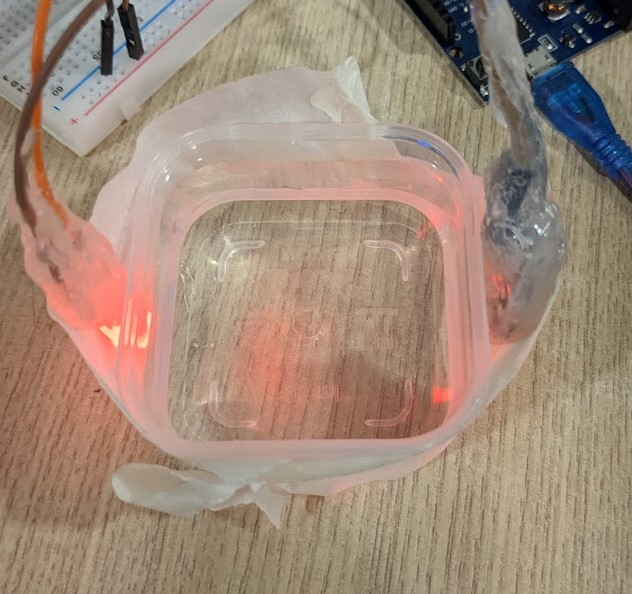
\includegraphics[width=0.8\linewidth]{report/images/clear_water.jpg}
        \caption{Clear Water}
        \textsc{Brightness Detected: 76\%}
    \end{subfigure}
    \begin{subfigure}{.33\textwidth}
        \centering
        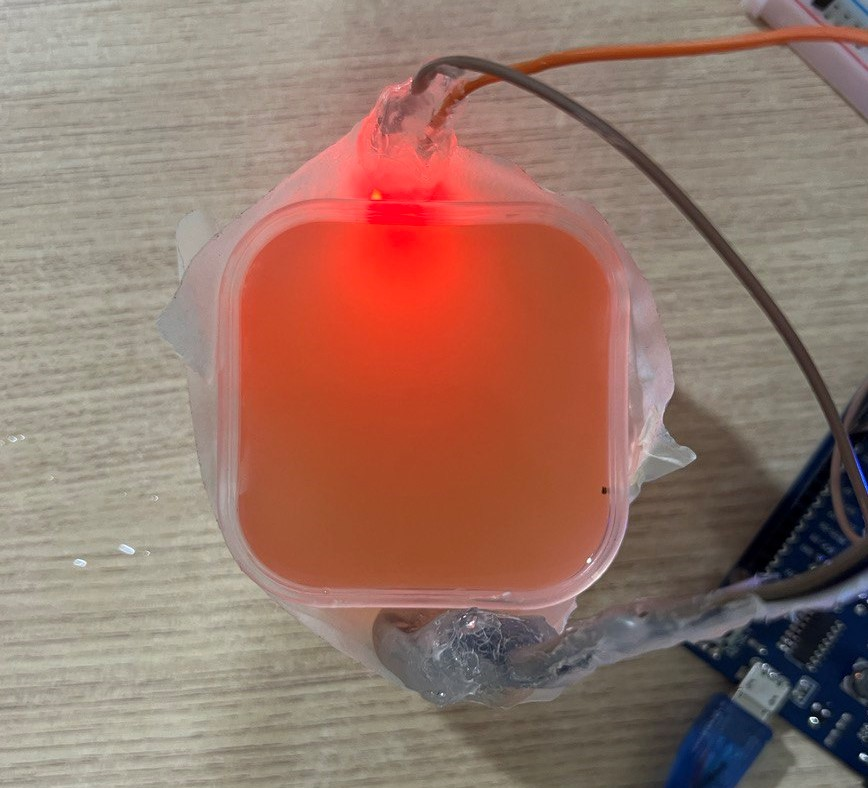
\includegraphics[width=.8\linewidth]{report/images/murky_water_mediocre.jpg}
        \caption{Water with 2 teaspoons of coffee}
        \textsc{Brightness Detected: 24\%}
    \end{subfigure}
    \begin{subfigure}{.33\textwidth}
        \centering
        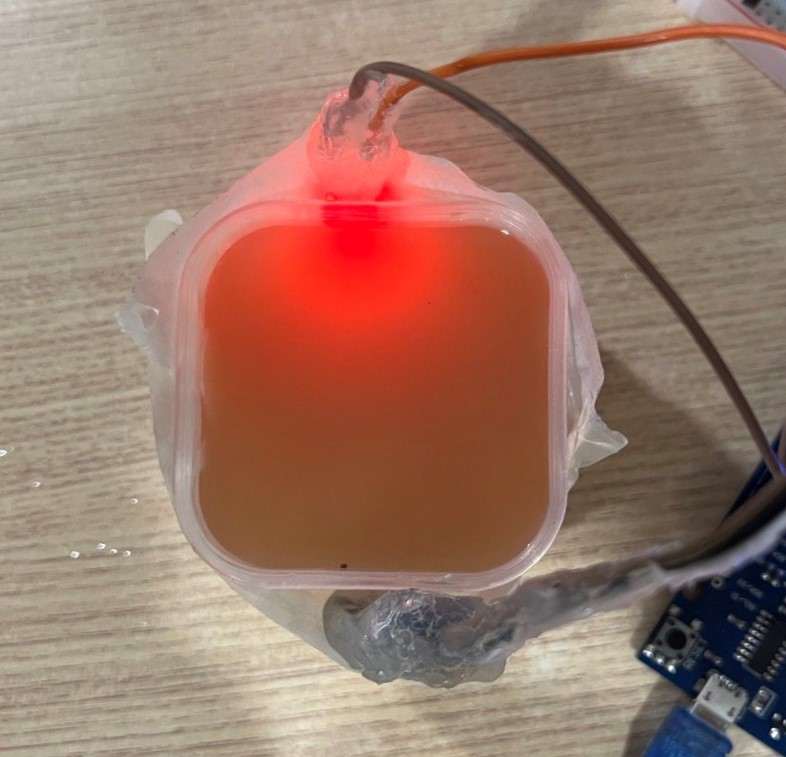
\includegraphics[width=.8\linewidth]{report/images/murky_water_very_poor.jpg}
        \caption{Water with 4 teaspoons of coffee}
        \textsc{Brightness Detected: 7.7\%}
    \end{subfigure}
\end{figure}

\subsection{Power modes and sampling frequencies}

One of the most important bottlenecks is obviously power supply, because the buoy must run on battery. To increase lifetime, we had the following idea:

\begin{multicols}{2}

\begin{_block}[]
Employ two different power modes:
\begin{enumerate}
    \item \textbf{intense}: high frequency data collection ($f_H$)
    \item \textbf{chill}: low frequency data collection ($f_L$)
\end{enumerate}
\end{_block}

The mode in which the buoy is currently is determined by the amplitude of the most recent measurement: if a value like g-force exceeds a hard-coded threshold and the buoy is currently in \textit{chill}, it switches to \textit{intense}. Doing so it also sends a wake up call over MQTT to any other buoys who are listening, but receiving the messages unfortunately didn't work on the WeMOS.

For simplicity- and demo-purposes we chose $f_H=1Hz$ and $f_L=0.1Hz$.

Using different data collection intensity modes suggests employing different power modes of the WeMOS. Unfortunately, it was not feasible to put the WeMOS in \textit{light sleep mode} for the frequencies listed above. This is because \textit{light sleep mode} kills the WiFi connection between the WeMOS and phone, and reconnecting to the hotspot is unreliable and may take longer than the sampling frequency above.

\textit{Deep sleep mode} is not useful as well because it puts the whole WeMOS to sleep, including \ISquaredC\ devices. Given that the MPU shouldn't be moving when calibrating upon start-up, it is not feasible to restart the MPU while the buoy is in moving waters.

In real application one would probably significantly increase the delay in chill mode.

\begin{code}[c]{WeMOS scheduler}
<-snip->
namespace scheduler {
    int last_fetch;
    bool intense = true;
    int last_time_intense_detected = 0;
    
    void init() { <-snip-> }
    void set_intense(){ <-snip-> }
    void set_chill(){ <-snip-> }
    int get_delay(){ <-snip-> }

    // return delay time until next fetch
    void wait() { <-snip-> }
    
    // update mode based on most recent measurements
    // if amplitudes exceed threshold, wake up
    void update(float g_force, float brightness){ <-snip-> }
}
\end{code}

\end{multicols}

\newpage
\subsection{\ISquaredC\ Communication}

\begin{multicols}{2}

The communication between ADC, MPU, and WeMOS is based on \ISquaredC. We first tried to rely on well-engineered libraries for this, which didn't work out well initially - as there were subtle differences between the same components built by different manufacturers and we ran into tons of issues.

This caused us to write the code for the ADC ourselves (based on the Lab and the provided spec sheet), which worked well initially. However, after a while we again couldn't initialize any devices, as register assignments to multiplex the analog ports seemed to switch randomly sometimes. We eventually managed to get it working using the \lstinline{ADS1115_WE} library.

For the MPU we ended up using the \lstinline{MPU6500_WE} library, which is impressively feature-rich.

The combination of MPU, ADC, and \ISquaredC\ made reading from the sensors mostly reliable and comparably easy to debug.

\begin{code}[c]{ADC \ISquaredC}
#include <ADS1115_WE.h>
namespace adc {
    <-snip->
    float read(int channel) {
        float voltage = 0.0;
        ADS1115_MUX c;
        switch (channel) {
            case 0: c = ADS1115_COMP_0_GND; break;
            <-snip->
        }
        _adc->setCompareChannels(c);
        _adc->startSingleMeasurement();
        while(_adc->isBusy()){}
        return _adc->getResult_V() / 3.3;
    }
}
\end{code}

\end{multicols}

\subsection{Buoy-Server}

\begin{multicols}{2}

The communication between buoy and server is based on MQTT. The broker is running on the server and an arbitrary number of phones from buoys can connect to it and start pushing data. The server stores the data in a MongoDB database, and has some services running to periodically run data updates and aggregations, see \textit{ML model and application}.

\end{multicols}

\subsection{Data collection}

\begin{multicols}{2}

As there were little to no data available for our project requirements, we had to collect the data ourselves. This posed several issues as we had to first find a good location to deploy our buoy, and then wait for good weather conditions. As aforementioned, we will only predict a score relative to our self-defined baseline for good weather conditions.

Due to the limited time we had for the project, we decided on West Coast Park in Singapore as our testing/deployment ground as it was the closest shoreline to the faculty. However, given that a major port is also situated at the location, waves from occasional passing tankers and ships could have affected the conditions for the baseline for the turbidity sensor. However, the location was still suitable for our purposes as the waters were deep and the site was relatively blocked by surrounding landmasses, allowing us to deploy the buoy in waves that are not breaking in shallow water. 

We deployed our buoy at the same location across 2 days as part of our data collection process. The outcome of the data collection process is shown in the chart below. It is possible to observe from the accelerometer data that there were moderate waves throughout our period of data collection. We would also like to point out that there were anomalous data collected, such as ourselves moving the buoy while in the process of deploying it into the sea. These outliers resulted in a particular challenge in the training process later, as we had to filter out the outlying data first.

Another issue faced throughout our data collection process was the weather. Throughout the data-collection phase, the weather remained fairly calm and sunny. 
Given time constraints at hand, we did not have the opportunity to gather data relating to bad weather conditions and diving condition. We recognise that this may not be the most optimal way to collect data as we can only classify our observations into one category. If properly deploying this system, it would be extremely beneficial to collect more extensive data over several days and across varying conditions in order to build a model that recognizes and predict different types of weather and conditions 


\begin{figure}[H]
    \centering
     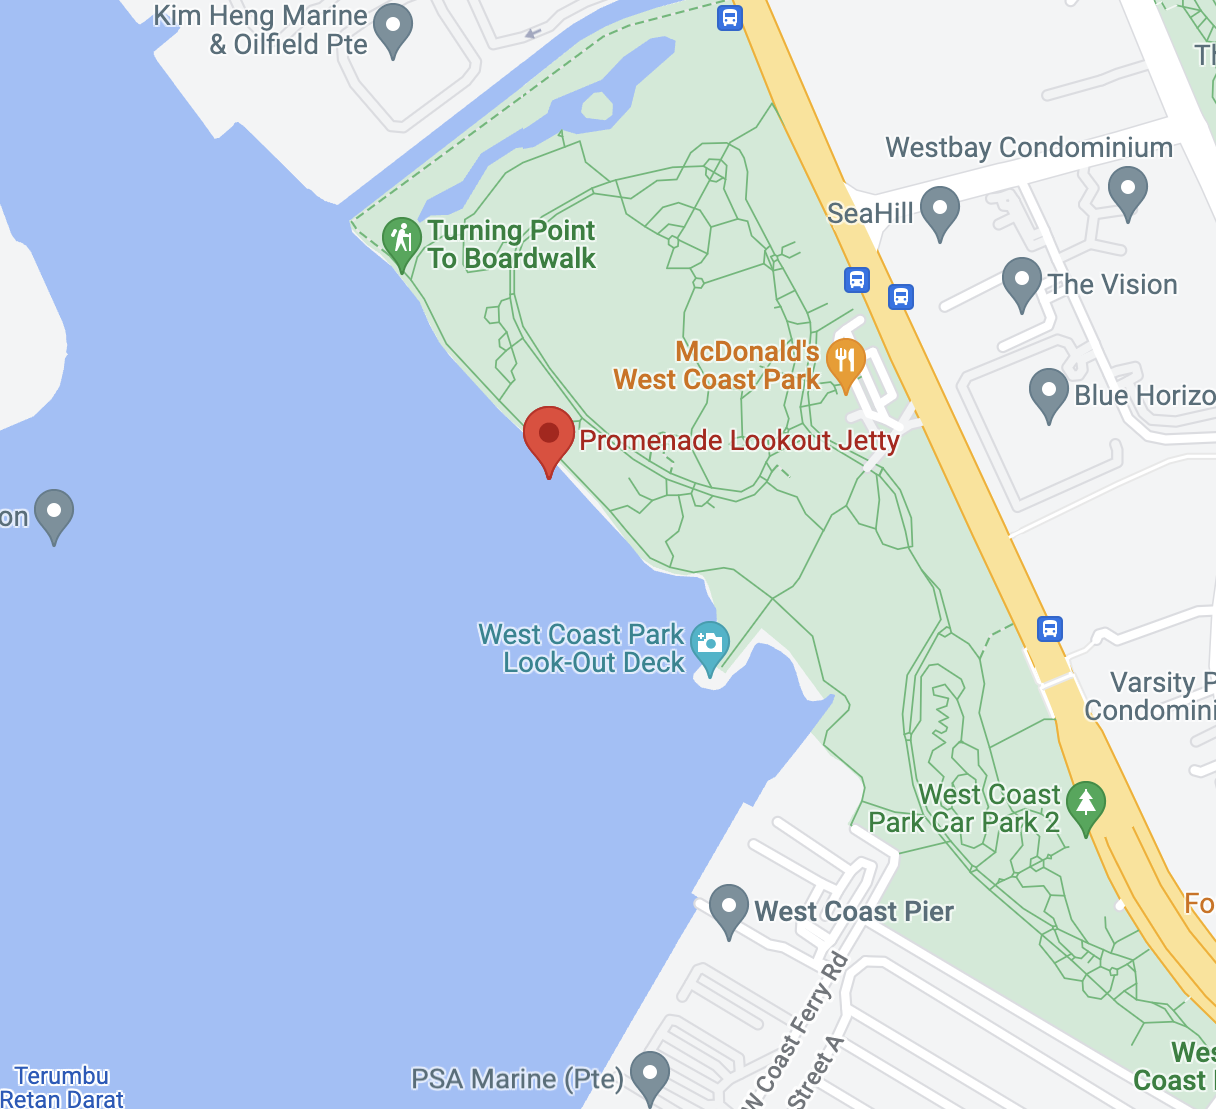
\includegraphics[height=8cm]{report/images/datacollection_location.png}
    \textsc{West-Coast Park: Collection spot (Google Maps)}
\end{figure}
% \begin{center}
%  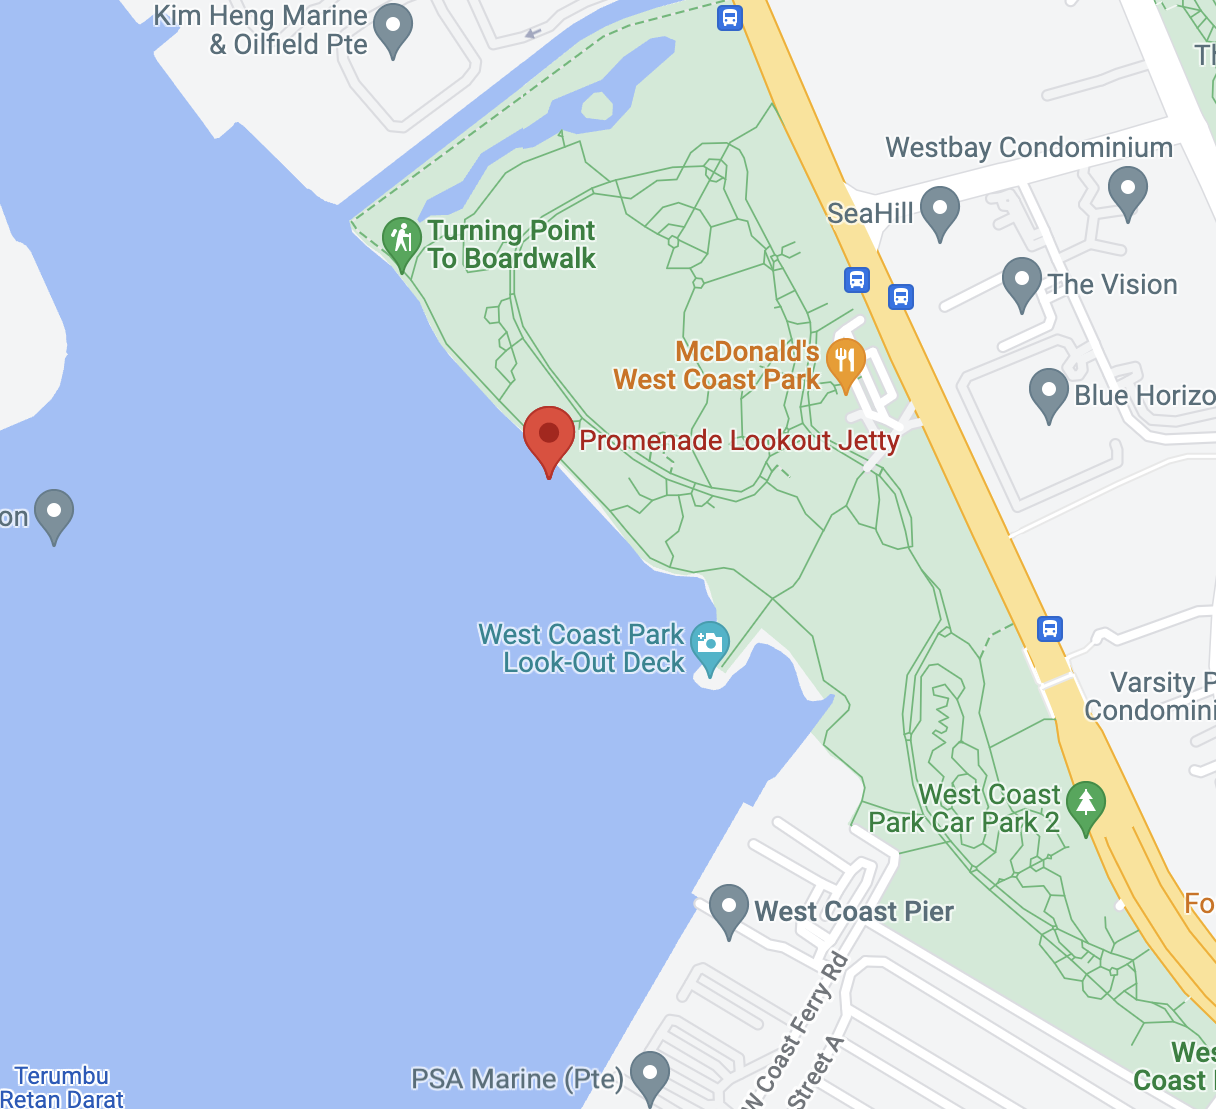
\includegraphics[height=\columnwidth]{report/images/datacollection_location.png}\\
% \textsc{West-Coast Park: data collection spot\\Source: Google Maps}
% \end{center}
% \begin{center}
%      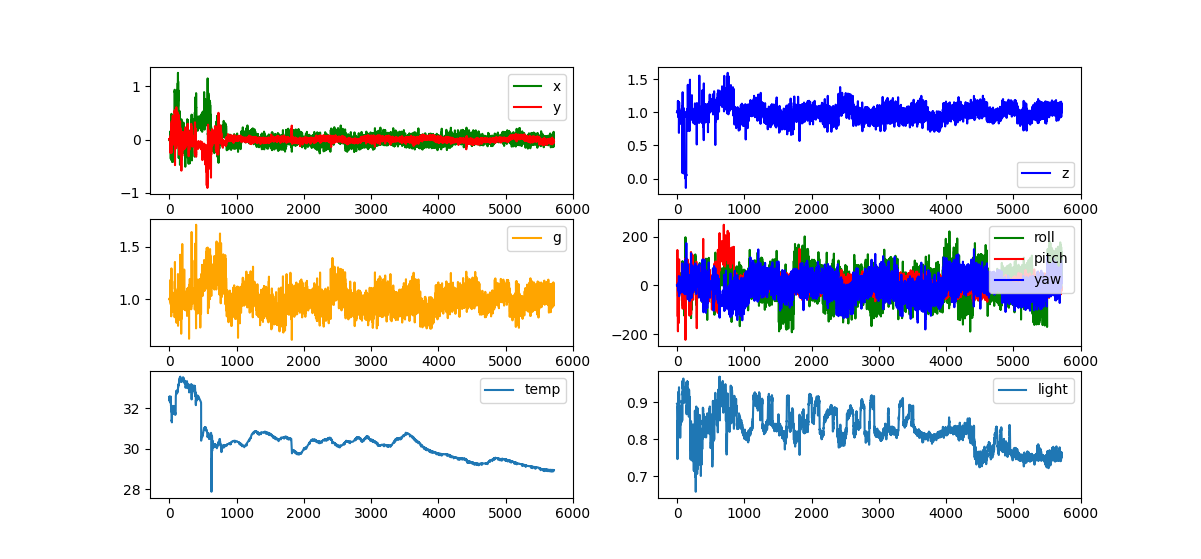
\includegraphics[width=\columnwidth]{report/images/good_data.png}\\
%      \textsc{Sample data we collected}
% \end{center}

\end{multicols}

\begin{figure}[H]
    \centering
    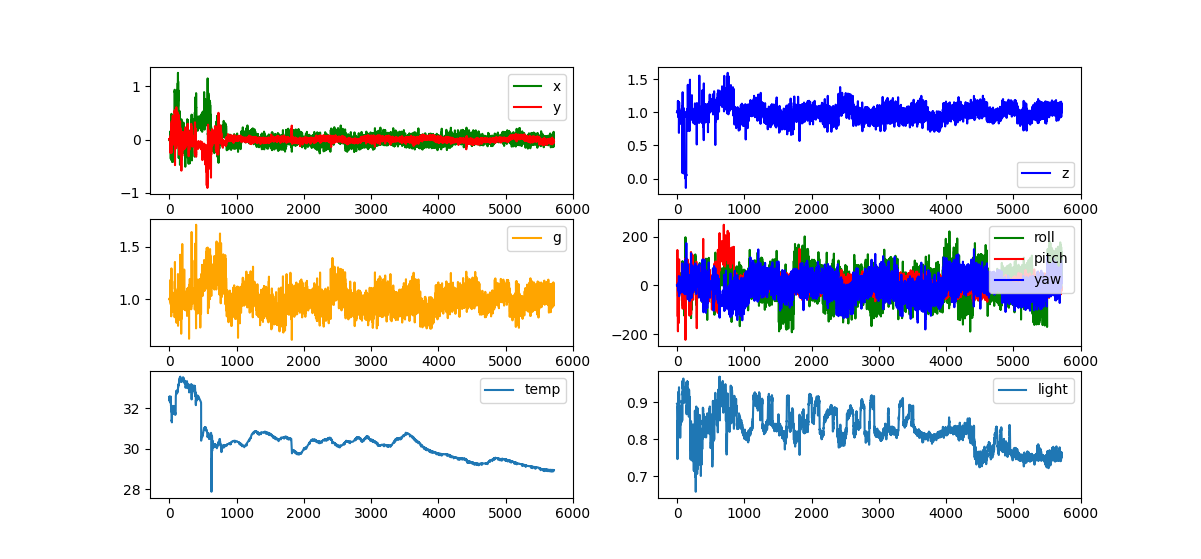
\includegraphics[width=\textwidth]{report/images/good_data.png}
    \textsc{Visualization of data collected data}
    \label{fig:my_label}
\end{figure}
\section{Experimental Evaluation}

\subsection{Model accuracy}

\begin{multicols}{2}
    
The accuracy of our LSTM models were tested by splitting our availabile data into training and testing subsets, then calculating the RMSE of both the testing and training datasets. We note that the RMSE scores between testing and training datasets for each of the LSTM models for turbulence, light and temperature do not convey high accuracy. However, we believe that the accuracy of our LSTM models can be improved with a greater amount of data collected from our buoys before training them.

\end{multicols}
\begin{figure}[H]
    \centering
    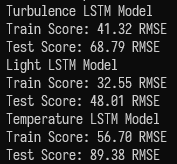
\includegraphics[width=5cm]{report/images/rmse.png}\\
    \textsc{RMSE of LSTM Models}
    \label{fig:my_label}
\end{figure}
% \begin{center}
%      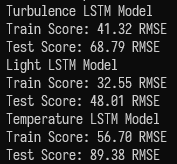
\includegraphics[width=5cm]{report/images/rmse.png}\\
%      \textsc{RMSE of LSTM Models}
% \end{center}


\newpage
\section{Challenges and Outlook}

\subsection{Phone reliance}
\begin{multicols}{2}
Using the phone as a middle-man between the WeMOS and cloud may introduce additional points of failure into our IoT solution. Such points of failure may include the phone running out of battery, or the application not working as intended due to Android/iOS aggressively preventing the application from running in the background, etc.

In our project, some aspects of the phone can be removed if given a wider variety of sensors. For example, a GPS module can replace the GPS data from the phone. A real time clock module can be used to replace the time information from the phone. Data can also possibly be buffered on the WeMOS instead of the phone before being pushed to the cloud, bypassing the phone. As such, in such a scenario, the phone simply acts as a gateway, providing internet connection to the WeMOS, simplifying our architecture.

% \columnbreak
% \begin{figure}[H]
%     \centering
%     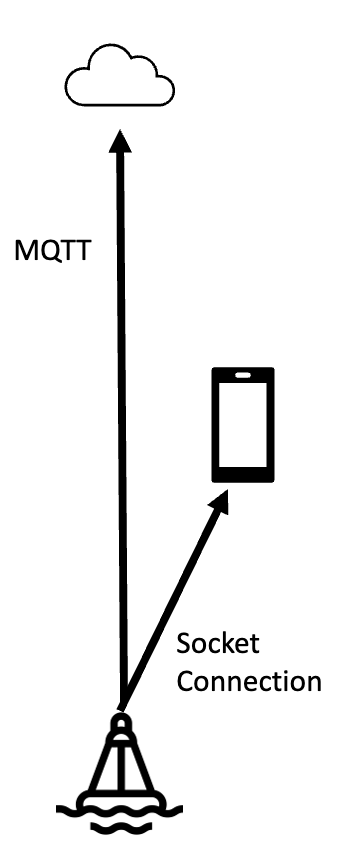
\includegraphics[height=10cm]{report/images/alternative_phone_wemos.png}
%     \text{Device Connection Diagram}
% \end{figure}
% \begin{center}
%  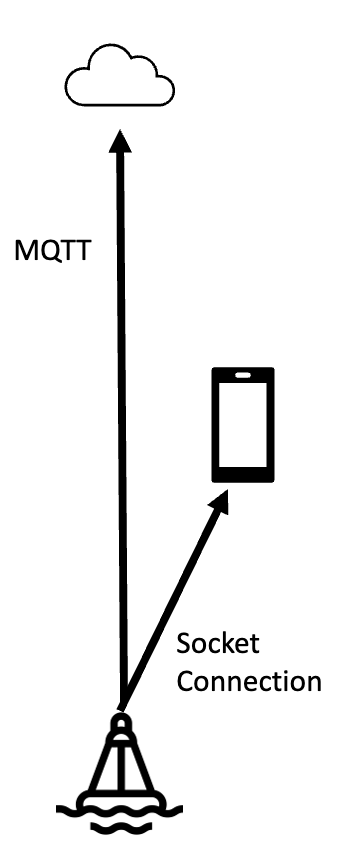
\includegraphics[height=10cm]{report/images/alternative_phone_wemos.png}\\
% \textsc{Device Connection Diagram}
% \end{center}

\end{multicols}

\subsection{Data bottleneck}

\begin{multicols}{2}
Our team faced challenges with collecting sufficient training data due to time constraints. There was also not many other sources of data applicable to our project online. We managed to only collect data on two separate days. Further, our data collected was bound to the West Coast geographical area during calm weather conditions. This may have affected the generalisability of our forecasts. With a greater budget to purchase water-rated sensors and more time to collect data, our model could have been made more reliable. An increased budget may also allow us to perform data collection safely during stormy conditions.
\end{multicols}

\subsection{Alternative Statistical methods}

\begin{multicols}{2}
 Statistical methods can be used to characterize the turbulence of the water, which in turn may be useful in generating a diver-safety score.

 Let $X$ be a random variable denoting the readings from an accelerometer. Given a sequence of accelerometer readings $x_1, x_2, ..., x_n$ at random intervals, the variance of $X$ can be used to give a score to the turbulence of the water. When stationary, no force is exerted upon the buoy and the accelerometer will give a constant output for each measurement, and hence $Var(X) = 0$. In calm waters, the accelerometer will register a range of values from stationary to slight accelerations depending where the measurement was taken during the wave. For choppy waters, the forces exerted upon the buoy are greater and will register a larger range of accelerations, and we can expect $Var(X_{stationary}) < Var(X_{calm}) < Var(X_{choppy})$. A variance of the last $n$ most recent readings will be useful in characterizing the choppiness of the water.
\end{multicols}


\section{Conclusion}


    Other than to provide a diving warning system, we can re-purpose our buoys for other tasks. Through this project, we have demonstrated the potential in collecting useful maritime data using cheap sensors. Data collected from the buoys, such as localised wave turbulence, water visibility and temperature are useful in maritime research. More complicated sensors such as water quality sensors or even cameras can be added to the buoy as well. 


% \subsection{Acknowledgements}
% \begin{multicols}
% \end{multicols}


\end{document}